\section{Summary}

\subsection{Data source}


Canadian oceans provide an important source of livelihood to Canadian in addition to fulfilling many important ecological roles.
The Canadian Government has a mandate to ensure the Oceans remain ecologically healthy as well as economically viable.
The Department of Fisheries and Oceans (DFO) is tasked with conducting regular stock assessments surveys to monitor the populations of fish and other aquatic
organisms, including crustaceans.
These surveys are carried out on either Canadian Coast Guard Science vessels or contracted out through privately owned fishing vessels.
Across Canada, fishing is conducted using a variety of gear types.
In the southern Gulf of St. Lawrence, fishing is primarily carried out using bottom trawls.
In addition to biomass data, oceanographic measurements, such as water salinity, temperature and dissolved oxygen, are often collected.
The ultimate goal of these surveys is to estimate population indices for species of ecological and economic interest.
Many of the data from stock assessment surveys have been made available via the Open Government Portal~\cite{ogp}.


The importance of having robust models for predicting the distribution of aquatic organisms cannot be overstated.
From a resource extraction point of view, modelled distributions can help direct fishing efforts; resulting in more efficient fisheries.
From an environmental conservation point of view, distributions modelling can help to identify which geographic areas should be targets for
conservation efforts.
The goal of this analysis is to compute models that can be used to predict the probability of occurrences of species of interest in the Southern
Gulf of St. Lawrence (sGSL).
Specifically, I employ a logistic regression approach, using latitude, longitude and water depth (i.e., elevation) to predict the probability of
occurrence of the following six species:

\begin{itemize}
    \item American plaice (\textit{Hippoglossoides platessoides})
    \item Atlantic cod (\textit{Gadus morhua})
    \item Atlantic herring (\textit{Clupea harengus})
    \item Redfish unidentified (\textit{Sebastes sp.})
    \item American lobster (\textit{Homarus americanus})
    \item Snow crab (\textit{Chionoecetes opilio})
\end{itemize}

The primary dataset used originating from the Government of Canada's Open Government Portal~\cite{ogp}, is a dataset called
\textbf{NAFO Division 4T groundfish research vessel trawl survey (September Survey) dataset}~\cite{groundfish}.
This dataset contained information biological information (i.e., species caught, specimen counts and specimen weights),
fishing information (i.e., gear type used, fishing vessel) and geospatial information (i.e., latitude and longitude).
Bathymetric data for the sGSL was obtained from the \textbf{General bathymetric Chart of the Oceans (GEBCO)}~\cite{gebco} website.


\subsection{Analysis}

The material in the course modules on Logistic Regression provided a useful starting point for this analysis.
This analysis had a strong spatial component and it took me lots of time to figure out how to properly re-project a geographical dataset
from one coordinate reference system to another.
The operations on the large data arrays for elevation and probability of occurrence were done using the \textbd{Xarray} python package~\cite{xarray}.
This was my first time using this package and while it was very impressive and comprehensive, it was also somewhat overwhelming.
It took me a long time to figure out how to extract the data from a data array, manipulate it and create a new data array.
A combination of persistence and stack overflow helped me to overcome these challanges.

\subsection{Conclusions}

The distribution models of the six species demonstrated different patterns of occurrence; some being more heterogeneous than others.
Species like American plaice and Atlantic cod were generally observed to be ubiquitous in the sGSL, especially in the shallower waters.
For those species, there is a much lower probability of occurrence in the deeper waters of the St. Lawrence seaway.
The modeled distributions of Atlantic herring and Snow crab seemed to be more influenced by latitude-longitude than by elevation.
Redfish and American lobster had sharp signals of presence-absence, i.e., a relatively narrow range of inflection in the sigmoid
logit(p) vs. p plots.
The distribution of both of these species seemed heavily driven by elevation, albeit inversely from one another.
Redfish were predicted to occur primarily in deep waters and lobster were predicted to occur primarily in shallow waters.
This in fact matches reality very closes, as can be observed by the overlaid points on the heatmaps in Figure~\ref{fig:heat_maps} below.



\begin{figure}
    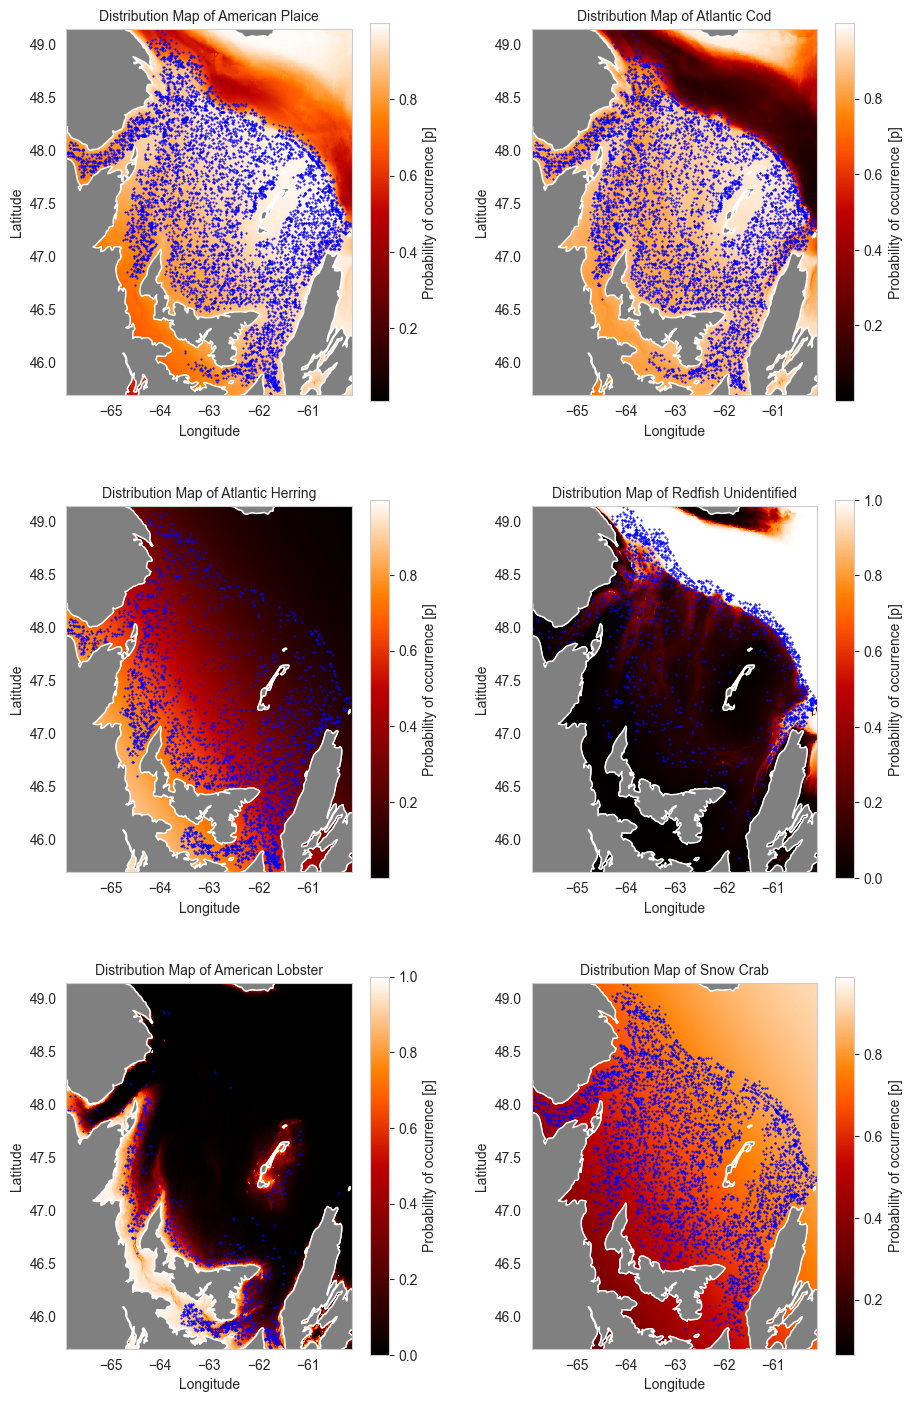
\includegraphics[height=18cm,keepaspectratio]{heat_maps}
    \caption{
        Distribution maps for all six species.
        Each map displays the inferred estimated probability for each point on the map and is depicted using a heatmap themed color mapping.
        The true occurrences for each species are overlain in order to provide a visual sense of model's performance.
    }
    \label{fig:heat_maps}
\end{figure}